\documentclass[10pt,a4paper]{article}
\usepackage[utf8]{inputenc}
\usepackage[T1]{fontenc}
\usepackage{lmodern}
\usepackage[margin=1.5cm, top=1.4cm, bottom=1.4cm]{geometry}
\usepackage{hyperref}
\usepackage{enumitem}
\usepackage{titlesec}
\usepackage{xcolor}
\usepackage{graphicx}

\definecolor{accent}{HTML}{00686E}
\hypersetup{colorlinks=true, urlcolor=accent, linkcolor=accent}
\pagenumbering{arabic}
\setlength{\parindent}{0pt}

\titleformat{\section}{\large\bfseries\color{accent}}{}{0em}{}[\vspace{-0.6em}\rule{\textwidth}{0.8pt}]
\titlespacing{\section}{0pt}{7pt}{4pt}

\newcommand{\role}[4]{%
  \textbf{#1} \hfill \textbf{#2}\\[1pt]%
  \textit{#3} \hfill \textit{#4}\\[2pt]%
}
\setlist[itemize]{leftmargin=1.2em, itemsep=1.5pt, topsep=2pt, parsep=0pt}

\begin{document}

% ================= HEADER =================
\begin{minipage}[c]{0.80\textwidth}
  {\Huge\bfseries Prabhavit Gupta}\\[3pt]
  {\color{accent}\large Senior Infrastructure \& Security Engineer: GCP, Terraform \& SRE}\\[6pt]
  {\footnotesize +39 351 610 7807 ~$\vert$~
  \href{mailto:prabhavitg@gmail.com}{prabhavitg@gmail.com} ~$\vert$~
  \href{https://www.linkedin.com/in/prabhavit/}{linkedin.com/in/prabhavit} ~$\vert$~
  \href{https://github.com/prab-gupta}{github.com/prab-gupta} ~$\vert$~
  Venice, Italy (CET Time Zone / EU Permanent Resident / Unrestricted EU Work Authorization)}
\end{minipage}\hfill
\begin{minipage}[c]{0.18\textwidth}
  \raggedleft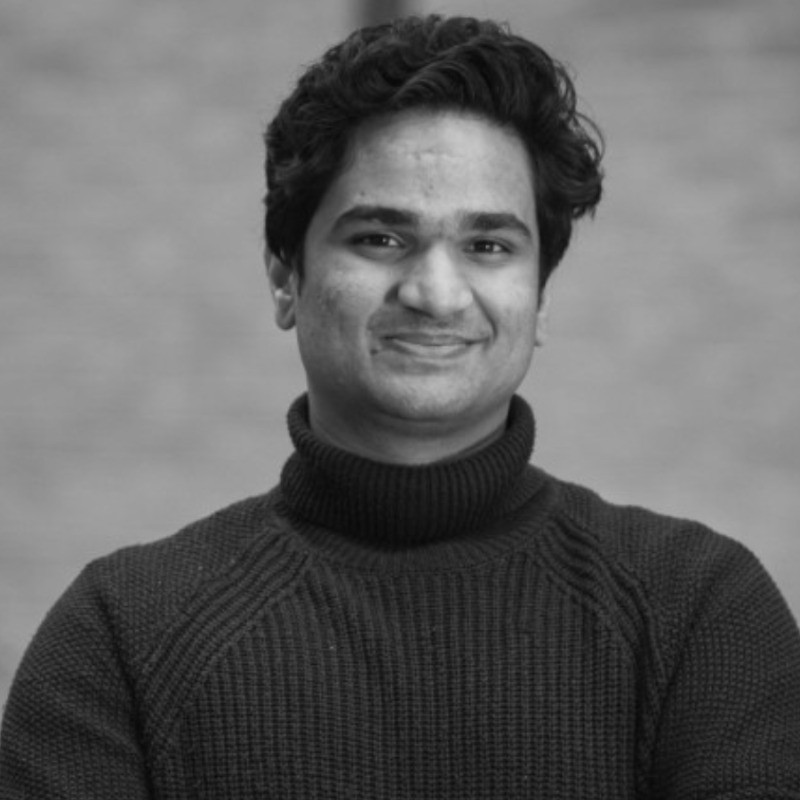
\includegraphics[width=2.0cm]{photo.jpg}
\end{minipage}
\vspace{-2pt}

% ================= SUMMARY =================
\section{Summary}
Senior Infrastructure, Platform, and Security Engineer with 3 years of commercial production experience designing, automating, and maintaining cloud platforms on Google Cloud Platform (GCP), Terraform infrastructure-as-code, and resilient SRE operations. Proven track record architecting secure multi-tenant microservices on GCP (Cloud Run, Cloud SQL, GCS, IAM, Secret Manager), implementing zero-trust network boundaries, and automating security-compliant CI/CD pipelines via GitHub Actions. Experienced engineering audit-ready compliance postures (SOC 2, ISO 27001 evidence automation, vulnerability scanning) and observability stacks delivering 99.8\% uptime. Based in Venice, Italy (CET time zone, matching Paris) with an EU Long-Term Residence Permit (permanent unrestricted EU work authorization across France and all EU member states, no visa sponsorship required); available immediately for full-time remote roles.

% ================= TECHNICAL EXPERTISE =================
\section{Technical Expertise}
\begin{itemize}
  \item \textbf{GCP Cloud Infrastructure:} Google Cloud Platform (GCP), Cloud Run, Cloud SQL, Google Cloud Storage (GCS), Secret Manager, IAM least-privilege policies, VPC networking, Cloud Armor, GKE.
  \item \textbf{Infrastructure as Code (IaC):} Terraform (production module design, state management, drift detection, automated plan validation), Docker containerization, Linux systems internals.
  \item \textbf{Security \& Compliance:} SOC 2 / ISO 27001 audit evidence automation, vulnerability management, dependency scanning (Trivy, Dependabot), TLS/PKI encryption in transit and at rest.
  \item \textbf{CI/CD \& SRE Operations:} GitHub Actions workflows, blue/green deployments, automated rollbacks, Prometheus and Grafana telemetry, SLO/SLI definition, structured JSON logging.
  \item \textbf{Languages \& Backend:} Python (FastAPI, asyncio, scripts), TypeScript/Node.js, SQL (PostgreSQL query optimization, partitioning), Bash shell automation.
  \item \textbf{Languages \& Work Authorization:} English (C1 Professional, fluent), Hindi (Native), Italian (Conversational). EU Long-Term Residence Permit (unrestricted EU work authorization across all EU countries, no sponsorship required).
\end{itemize}

% ================= EXPERIENCE =================
\section{Experience}

\role{\href{https://flowspace.co}{FlowSpace.co}}{Mar 2024 - Aug 2026}{Lead Infrastructure, Security \& Platform Engineer}{London, UK (remote)}
\begin{itemize}
  \item Architected and maintained the complete production GCP cloud footprint using Terraform, provisioning Cloud Run services, managed Cloud SQL instances, IAM security boundaries, and VPC networks.
  \item Established automated GitHub Actions CI/CD deployment pipelines with built-in SAST security scans, secret masking, and progressive zero-downtime releases for 4,500+ enterprise users.
  \item Implemented SOC 2 compliant operational safeguards including automated access review logging, encrypted storage buckets, Secret Manager rotation, and tamper-evident audit trails.
  \item Configured end-to-end platform observability using Prometheus, structured cloud logging, and automated alerting, sustaining 99.8\% production availability against strict SLAs.
  \item Hardened microservice Docker container images and network ingress rules, decreasing platform vulnerability exposure to zero critical CVEs.
\end{itemize}

\role{Urlink}{Apr 2025 - Jul 2025}{Cloud Platform \& Security Developer (Freelance)}{Barcelona, Spain (remote)}
\begin{itemize}
  \item Automated multi-environment cloud infrastructure provisioning across staging and production using modular Terraform configurations and Docker.
  \item Configured automated database encryption, automated backup verification, and disaster recovery procedures for enterprise customer data.
  \item Built automated integration test suites and security contract tests using pytest and Playwright to validate security headers, authentication cookies, and API authorization controls.
\end{itemize}

\role{Independent Technical Consultant}{Aug 2023 - Feb 2024}{Cloud Infrastructure \& Systems Engineer}{Venice, Italy}
\begin{itemize}
  \item Deployed secure cloud architectures and automated webhook microservices for European SMB clients, enforcing TLS termination and secret isolation.
  \item Implemented database migration pipelines, automated backup cron jobs, and Linux systemd monitoring daemons.
  \item Produced comprehensive infrastructure documentation, disaster recovery runbooks, and security compliance matrices for client engineering leadership.
\end{itemize}

% ================= EDUCATION =================
\section{Education}
\role{Ca' Foscari University of Venice}{2020 - 2024}{BA in Philosophy, International Studies and Economics}{Venice, Italy}
\begin{itemize}
  \item Rigorous training in formal logic, statistical inference, quantitative economics, and complex systems modeling.
\end{itemize}

\end{document}
